\documentclass[12pt,a4paper]{extarticle}
\usepackage[utf8]{inputenc}
\usepackage[T5]{fontenc}
\usepackage{geometry}
\geometry{a4paper, left=1.5cm, right=1cm, top=1.5cm, bottom=1.5cm, headheight=20pt, headsep=15pt, footskip=28pt}
\usepackage{enumitem}
\usepackage{amsmath}
\usepackage{amssymb}
\usepackage{diagbox}
\usepackage{colortbl} % Sửa lỗi \arrayrulecolor
\usepackage{array}    % Hỗ trợ định dạng cột m{2cm}
\usepackage[most]{tcolorbox}
\newcommand{\khongxacdinh}{\text{KXĐ}}
\newcommand{\blackbox}[1]{\texorpdfstring{\fcolorbox{black}{black}{\textcolor{white}{#1}}}{#1}}
\usepackage{tikz}
\definecolor{bookblue}{RGB}{58,90,172}
\definecolor{book}{RGB}{58,90,172}
\definecolor{myblue}{RGB}{200,40,40}
\newcommand{\bluecheck}{\textcolor{myblue}{\checkmark}}
\newtcolorbox{formulaBox}{colback=gray!5,colframe=bookblue,boxrule=0.8pt,arc=2mm}
\newtcolorbox{notebox}{colback=blue!3,colframe=myblue,boxrule=0.8pt,arc=2mm}
\usetikzlibrary{patterns, patterns.meta} % Thêm patterns.meta vào đây
% Gọi package nằm trong thư mục con template
\usepackage{../template/mngocbox}

\begin{document}

% Sử dụng ngoặc vuông [...] để thay đổi linh hoạt các thông số
\makeheadbox[headerright={Chương 5},chude={Bài 3},tieude={Phương trình mặt cầu},dinhdang={Hình học},lop={12 },gv={Nguyễn Lê Minh Ngọc}]
\vspace{2em}
\section*{\color{myblue}{A. KIẾN THỨC NỀN TẢNG}}
\begin{tcolorbox}[colback=lightblue, colframe=myblue, arc=2mm]
\noindent $\star$ Trong không gian $Oxyz$, phương trình mặt cầu $(S)$ có tâm $I(a; b; c)$ và bán kính $R$ là:
\[
(x - a)^2 + (y - b)^2 + (z - c)^2 = R^2
\]
Đặc biệt, mặt cầu có tâm là gốc tọa độ $O$ và bán kính $R$ có phương trình: $x^2 + y^2 + z^2 = R^2$.
\end{tcolorbox}
\vspace{0.3cm}
\begin{tcolorbox}[colback=lightblue, colframe=myblue, arc=2mm]
\noindent $\star$ Trong không gian $Oxyz$, phương trình có dạng:
\[
x^2 + y^2 + z^2 + ax + by + cz + d = 0
\]
là phương trình của một mặt cầu khi và chỉ khi $\dfrac{a^2}{4} + \dfrac{b^2}{4} + \dfrac{c^2}{4} - d > 0$. Khi đó tâm mặt cầu là:
\[
I\left(-\frac{a}{2}; -\frac{b}{2}; -\frac{c}{2}\right), \quad \text{bán kính } R = \sqrt{\frac{a^2}{4} + \frac{b^2}{4} + \frac{c^2}{4} - d}.
\]
\end{tcolorbox}
\vspace{0.3cm}
\begin{tcolorbox}[colback=lightblue, colframe=myblue, arc=2mm]
\noindent $\star$ Trong không gian $Oxyz$, cho 3 điểm $A(a; 0; 0), B(0; b; 0)$ và $C(0; 0; c)$ với $abc \neq 0$. Tâm mặt cầu ngoại tiếp tứ diện $OABC$ là:
\[
I\left(\frac{a}{2}; \frac{b}{2}; \frac{c}{2}\right).
\]
\end{tcolorbox}
\vspace{0.3cm}
\begin{tcolorbox}[colback=lightblue, colframe=myblue, arc=2mm]
\noindent $\star$ Trong không gian $Oxyz$, ta xét điểm $I(a; b; c)$ và đường thẳng $d: \begin{cases} \text{Qua } M(x_0; y_0; z_0) \\ \text{VTCP } \vec{u} = (m; n; p) \end{cases}$
\vspace{0.2cm}
Khoảng cách từ $I$ tới $d$ là:
\[
d(I, d) = \frac{\left|[\vec{u}, \vec{IM}]\right|}{|\vec{u}|}
\]
\textit{Công thức này giúp ta giải nhanh một số bài toán liên quan tới đường thẳng cắt mặt cầu.}
\end{tcolorbox}
\section*{\color{myblue}{Vị trí tương đối của mặt cầu}}
% ==================== A) ĐIỂM ====================
\subsection*{\color{myblue}{a) Vị trí tương đối giữa điểm và mặt cầu}}
\begin{tcolorbox}[colback=lightblue, colframe=myblue, arc=2mm]
Cho mặt cầu $(S)$ có tâm $I$, bán kính $R$ và điểm $M$:
\begin{itemize}
    \item $IM > R \implies$ \textbf{Điểm nằm ngoài mặt cầu}
    \item $IM = R \implies$ \textbf{Điểm nằm trên mặt cầu}
    \item $IM < R \implies$ \textbf{Điểm nằm trong mặt cầu}
\end{itemize}
\end{tcolorbox}
\vspace{0.3cm}
% ==================== B) ĐƯỜNG THẲNG ====================
\subsection*{\color{myblue}{b) Vị trí tương đối giữa đường thẳng và mặt cầu}}
\begin{tcolorbox}[colback=lightblue, colframe=myblue, arc=2mm]
Cho mặt cầu $(S)$ tâm $I$, bán kính $R$ và đường thẳng $\Delta$:
\begin{itemize}
    \item $d(I, \Delta) > R \implies$ \textbf{Không có điểm chung}
    \item $d(I, \Delta) = R \implies$ \textbf{Tiếp xúc} (đường thẳng là tiếp tuyến của mặt cầu)
    \item $d(I, \Delta) < R \implies$ \textbf{Cắt nhau} tại 2 điểm phân biệt $A, B$.
\end{itemize}
\vspace{0.2cm}
\noindent \textbf{Công thức liên hệ (Pythagoras):}
\[
d^2(I, \Delta) + \frac{1}{4} AB^2 = R^2
\]
\end{tcolorbox}
\vspace{0.3cm}
% ==================== C) MẶT PHẲNG ====================
\subsection*{\color{myblue}{c) Vị trí tương đối giữa mặt phẳng và mặt cầu}}
\begin{tcolorbox}[colback=lightblue, colframe=myblue, arc=2mm]
Cho mặt cầu $(S)$ tâm $I$, bán kính $R$ và mặt phẳng $(P)$:
\begin{itemize}
    \item $d(I, (P)) > R \implies$ \textbf{Không có điểm chung}
    \item $d(I, (P)) = R \implies$ \textbf{Tiếp xúc} (mặt phẳng là tiếp diện của mặt cầu)
    \item $d(I, (P)) < R \implies$ \textbf{Cắt nhau}, giao tuyến là một đường tròn bán kính $r$.
\end{itemize}
\vspace{0.2cm}
\noindent \textbf{Công thức liên hệ (Pythagoras):}
\[
d^2(I, (P)) + r^2 = R^2
\]
\end{tcolorbox}
\vspace{0.3cm}
% ==================== D) HAI MẶT CẦU ====================
\subsection*{\color{myblue}{d) Vị trí tương đối của hai mặt cầu}}
Cho hai mặt cầu $(S_1)$ tâm $I_1$, bán kính $R_1$ và $(S_2)$ tâm $I_2$, bán kính $R_2$:
\begin{tcolorbox}[colback=lightblue, colframe=myblue, arc=2mm]
\begin{center}
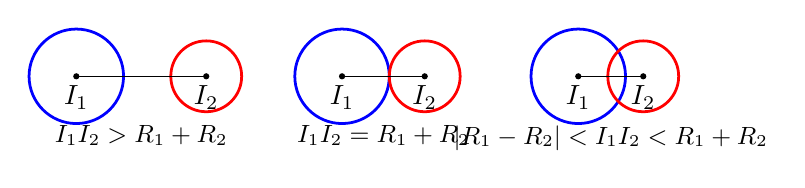
\begin{tikzpicture}[scale=0.75, >=stealth]
  % 1. Ở ngoài nhau
  \draw[blue, line width=1pt] (0,0) circle (0.8);
  \draw[red, line width=1pt] (2.2,0) circle (0.6);
  \draw (0,0) -- (2.2,0);
  \fill (0,0) circle (1.5pt) node[below] {$I_1$};
  \fill (2.2,0) circle (1.5pt) node[below] {$I_2$};
  \node[below=0.5cm, font=\small\bfseries] at (1.1,0) {$I_1I_2 > R_1 + R_2$};
  % 2. Tiếp xúc ngoài
  \draw[blue, line width=1pt] (4.5,0) circle (0.8);
  \draw[red, line width=1pt] (5.9,0) circle (0.6);
  \draw (4.5,0) -- (5.9,0);
  \fill (4.5,0) circle (1.5pt) node[below] {$I_1$};
  \fill (5.9,0) circle (1.5pt) node[below] {$I_2$};
  \node[below=0.5cm, font=\small\bfseries] at (5.2,0) {$I_1I_2 = R_1 + R_2$};
  % 3. Cắt nhau
  \draw[blue, line width=1pt] (8.5,0) circle (0.8);
  \draw[red, line width=1pt] (9.6,0) circle (0.6);
  \draw (8.5,0) -- (9.6,0);
  \fill (8.5,0) circle (1.5pt) node[below] {$I_1$};
  \fill (9.6,0) circle (1.5pt) node[below] {$I_2$};
  \node[below=0.5cm, font=\small\bfseries] at (9.05,0) {$|R_1 - R_2| < I_1I_2 < R_1 + R_2$};
\end{tikzpicture}
\vspace{0.4cm}
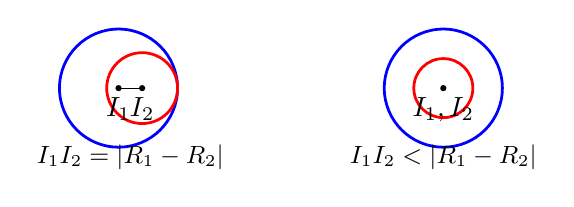
\begin{tikzpicture}[scale=0.75, >=stealth]
  % 4. Tiếp xúc trong
  \draw[blue, line width=1pt] (0,0) circle (1.0);
  \draw[red, line width=1pt] (0.4,0) circle (0.6);
  \draw (0,0) -- (0.4,0);
  \fill (0,0) circle (1.5pt) node[below] {$I_1$};
  \fill (0.4,0) circle (1.5pt) node[below] {$I_2$};
  \node[below=0.6cm, font=\small\bfseries] at (0.2,0) {$I_1I_2 = |R_1 - R_2|$};
  % 5. Ở trong nhau
  \draw[blue, line width=1pt] (5.5,0) circle (1.0);
  \draw[red, line width=1pt] (5.5,0) circle (0.5);
  \fill (5.5,0) circle (1.5pt) node[below] {$I_1, I_2$};
  \node[below=0.6cm, font=\small\bfseries] at (5.5,0) {$I_1I_2 < |R_1 - R_2|$};
\end{tikzpicture}
\end{center}
\end{tcolorbox}

\section*{\color{myblue}{Chùm mặt cầu}}
\subsubsection*{\color{myblue}{\underline{Kiến thức nền}}}
% ==================== TRƯỜNG HỢP 1 ====================
\begin{tcolorbox}[colback=lightblue, colframe=myblue, arc=2mm]
\begin{minipage}{0.4\textwidth}
\centering
% Hình vẽ TikZ 1: Giao của 2 mặt cầu và mặt phẳng gốc
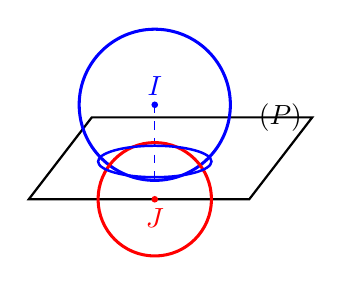
\begin{tikzpicture}[scale=0.8, >=stealth]
  % Mặt phẳng P
  \draw[line width=0.8pt] (-2,-0.5) -- (1.5,-0.5) -- (2.5,0.8) node[left] {$(P)$} -- (-1,0.8) -- cycle;
  
  % Mặt cầu S1 (Xanh)
  \draw[blue, line width=1.1pt] (0,1) circle (1.2);
  \fill[blue] (0,1) circle (1.5pt) node[above] {$I$};
  \draw[blue, dashed] (0,1) -- (0,-0.2);
  
  % Mặt cầu S2 (Đỏ)
  \draw[red, line width=1.1pt] (0,-0.5) circle (0.9);
  \fill[red] (0,-0.5) circle (1.5pt) node[below] {$J$};
  
  % Đường tròn giao tuyến E (nằm trên P)
  \draw[blue, line width=0.9pt] (0,0.1) ellipse (0.9cm and 0.25cm);
\end{tikzpicture}
\end{minipage}
\hfill
\begin{minipage}{0.56\textwidth}
\textbf{1.} Cho 2 mặt cầu:
\[
(S): x^2 + y^2 + z^2 + ax + by + cz + d = 0
\]
\[
(S'): x^2 + y^2 + z^2 + a'x + b'y + c'z + d' = 0
\]
cắt nhau theo giao tuyến là đường tròn $(E)$.
\vspace{0.2cm}
Mặt phẳng $(P)$ chứa đường tròn giao tuyến $(E)$ có phương trình:
\[
\mathbf{(a-a')x + (b-b')y + (c-c')z + (d-d') = 0}
\]
\[
\mathbf{\Big( (S) - (S') = 0 \Big)}
\]
\end{minipage}
\end{tcolorbox}
\vspace{0.5cm}
% ==================== TRƯỜNG HỢP 2 ====================
\begin{tcolorbox}[colback=lightblue, colframe=myblue, arc=2mm]
\begin{minipage}{0.4\textwidth}
\centering
% Hình vẽ TikZ 2: Họ mặt cầu đi qua đường tròn giao tuyến
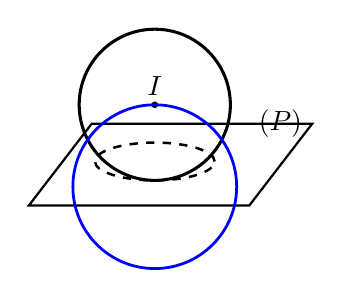
\begin{tikzpicture}[scale=0.8, >=stealth]
  % Mặt phẳng P
  \draw[line width=0.8pt] (-2,-0.5) -- (1.5,-0.5) -- (2.5,0.8) node[left] {$(P)$} -- (-1,0.8) -- cycle;
  
  % Mặt cầu S gốc (Đen)
  \draw[line width=1.1pt] (0,1.1) circle (1.2);
  \fill (0,1.1) circle (1.5pt) node[above] {$I$};
  
  % Đường tròn giao tuyến E
  \draw[dashed, line width=0.9pt] (0,0.2) ellipse (0.95cm and 0.3cm);
  
  % Mặt cầu thuộc chùm (Xanh dương)
  \draw[blue, line width=1pt] (0,-0.2) circle (1.3);
\end{tikzpicture}
\end{minipage}
\hfill
\begin{minipage}{0.56\textwidth}
\textbf{2.} Cho mặt phẳng $(P): ax + by + cz + d = 0$ và mặt cầu $(S): x^2 + y^2 + z^2 + Ax + By + Cz + D = 0$ cắt nhau theo giao tuyến là đường tròn $(E)$.
\vspace{0.2cm}
Tất cả các mặt cầu chứa đường tròn $(E)$ đều có phương trình dạng:
\[
\mathbf{x^2+y^2+z^2+Ax+By+Cz+D + m(ax+by+cz+d) = 0}
\]
\[
\mathbf{\Big( (S) + m(P) = 0 \Big)}
\]
\end{minipage}
\end{tcolorbox}
\end{document}